\documentclass[12pt, letterpaper]{article}
\usepackage[letterpaper, margin=1in]{geometry} % Decrease page margins
\title{ECE Project Proposal: Audio Effects Box}
\author{Anton Liakhovitch}

\usepackage{graphicx}
\graphicspath{{images/}}
\usepackage[defaultlines=4,all]{nowidow} % Discourage paragraph breaks across pages
\usepackage[skip=10pt plus1pt, indent=0pt]{parskip}
\usepackage[british]{babel}

\newcommand{\lbr}{\\[12pt]}
\renewcommand\labelitemi{--} % Use dashes in lists

\begin{document}
\maketitle
\section{Background}
\par
Music producers employ a variety of effects in order to improve or modify their audio. Effects normally take one of two forms: \textit{effects plugins}, and \textit{effects boxes} (also known as \textit{effects pedals}).
\par
An effect plugin is computer software which integrates with a \textit{digital audio workstation} (DAW) program via one of several standard plugin protocols. The DAW allows the producer to compose and record music, while plugins provide effects and other tools.
\par
An effects box is a physical device which normally includes at least one audio input and one audio output. The box applies a given effect to the incoming audio signal in real time. For example, a delay pedal might add in delayed copies of the original signal for an 'echo' effect. Many software plugins use 'virtual analog' algorithms to emulate well-known physical effects boxes.
\par
Sonic Charge - a music software company - makes an effect plugin called \textit{Permut8}. The user interface is visible in Figure~\ref{fig:permut8}. On the left, a virtual analog section allows for basic mixing and filtering operations. On the right side, a digital section allows for manipulation of the signal to create various 'glitch' effects. The plugin is intentially made to look and behave like an emulation of a physical effects box - however, no physical version of Permut8 has ever been built.


\section{Goal}
\par
This project aims to create a physical effects processing box with similar functionality to Sonic Charge's Permut8 software plugin. The scope of the project covers only the \textit{digital section} of Permut8; the 'virtual analog' section is mostly out of scope and may be added later through updated hardware or software.
\begin{figure}
  \centering
  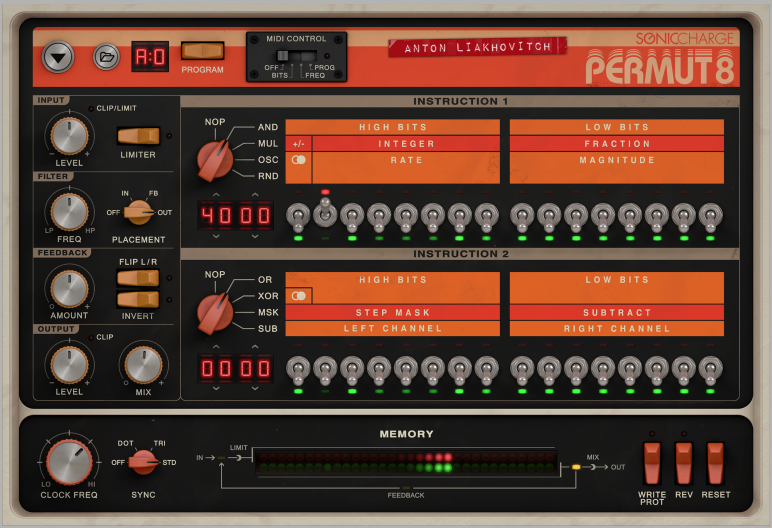
\includegraphics[width=0.8\textwidth]{permut8}
  \caption{Sonic Charge 'Permut8' Effects Plugin}
  \label{fig:permut8}
\end{figure}


\section{Functionality}
\par
Permut8, the original inspiration for this project, is a form of digital delay effect. The plugin is designed as a software emulation of a fictional piece of hardware. This section provides a brief summary of this fictional hardware. For detailed information, see the \textit{Permut8 User Guide}.
\subsection{Buffer}
\par
At the core of Permut8 is a memory buffer which stores 128,000 audio samples. The device is clocked at a variable rate, ranging from 0 to 352.8KHz. On each cycle, audio is sampled from the input and written to the buffer. Then, a sample is read from the buffer and sent to the output. The \textit{write address} increments by one every clock cycle and wraps around to zero at the end of the buffer. By default, the \textit{read address} is the same as the write address. Thus, by default, the plugin makes no changes to the incoming audio - it records an input sample into a buffer, then reads and outputs the same sample. In the interface (Figure~\ref{fig:permut8}), the read and write positions are visible on the 'LED bar' at the bottom.
\lbr
The behavior is analogous to a loop of tape, where a write head is placed immediately in front of a read head.
\subsection{Operations}
Permut8 can apply up to two \textit{operations} to the read address in order to make the output more interesting \footnote{The Permut8 manual refers to these operations as "instructions".}. For example, the "SUB" operator subtracts a fixed value from the read address. This makes the read position lag behind the write position by some amount of time, thereby delaying the output signal. The rows of switches seen in Figure~\ref{fig:permut8} configure input parameters for the operators.
\subsection{Mixer}
While the mixer is part of the 'virtual analog section', it is simple to emulate digitally. The mixer includes several controls:
\begin{itemize}
\item \textit{Output level} controls the output audio level.
\item \textit{Mix} controls how much of the original, unmodified signal is mixed into the output.
\item \textit{Feedback} controls how much of the output signal is mixed back into the input.
\end{itemize}
\section{Project Scope}
This project aims to implement most of the functionality of Permut8's 'digital' section, and some of the functionality of the 'analog' section. This includes:
\begin{itemize}
  \item The audio buffer.
  \item Both operators, with all available operations.
  \item Variable audio clock frequency \footnote{This refers to the processing algorithm only - it does not need to correspond to any actual hardware clock frequencies.}.
  \item Write protect, reverse, and reset switches.
  \item Stereo audio processing.
  \item The three mixer knobs (\textit{output level}, \textit{mix}, and \textit{feedback}).
  \item The 'invert' and 'flip L/R' switches for feedback.
\end{itemize}
Notable omissions:
\begin{itemize}
  \item The analog filter and limiter, and the input level knob.
  \item Tempo sync functionality.
  \item Preset-saving functionality.
  \item Hexadecimal operand indicator displays.
\end{itemize}
There are also additional requirements based on practical considerations of physical hardware development:
\begin{itemize}
  \item Standard connectors (1/4 inch or 1/8 inch TRS) for audio in/out)
  \item 16-bit or 32-bit DAC and ADC \footnote{The original Permut8 uses 12-bit audio. 24-bit is generally considered the highest resolution detectable by humans. However, extra resolution is useful in a hardware context because it allows for a wide range of input levels.}.
\end{itemize}


\section{Basic Design}
The draft design described here is subject to change, and should only be used to gain an understanding of the technologies and challenges involved in the project.
\par
The device will be based on a readily available 32-bit ARM MCU - for example, the STM32\-F411 or the RP\-2040. The MCU will communicate with a stereo ADC/DAC IC over an I2S (or similar) interface. The audio buffer will be stored in an external RAM module, connected via either a parallel or SPI interface. Buttons, knobs, and LEDs will be accessed via a chain of shift registers. Firmware will be written in Rust.
\begin{figure}[!ht]
  \centering
  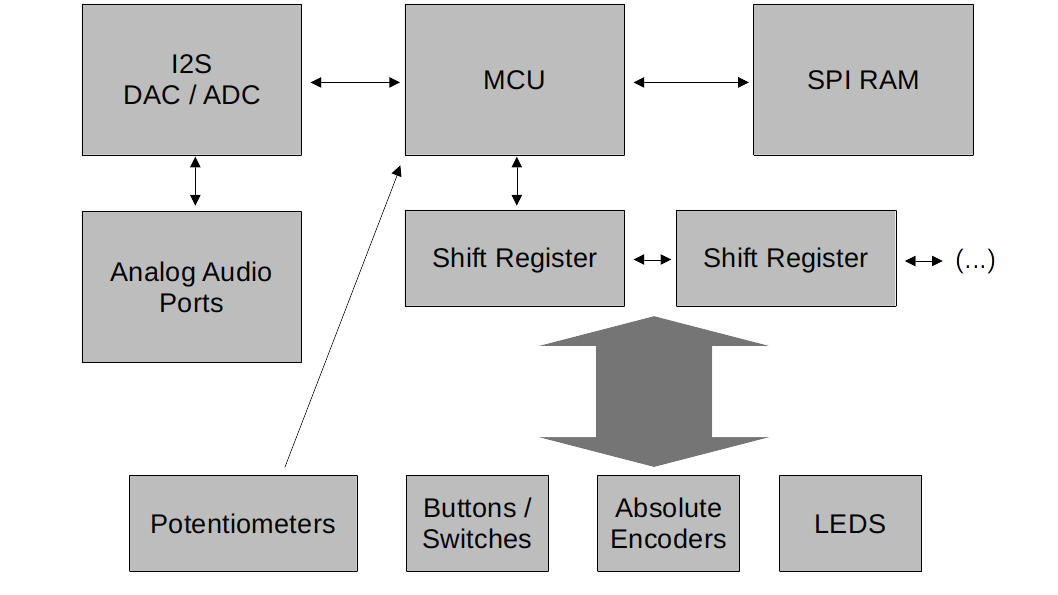
\includegraphics[width=1.0\textwidth]{block_diagram}
  \caption{High-level Hardware Diagram}
  \label{fig:block_diagram}
\end{figure}


\section{Optional Features}
Additional features may be added once the rest of the project is complete. These features are optional, and no time should be spent on them until the rest of the project is done - however, some consideration may be put into forwards compatibility so that they can be easily added later. Potential optional features include:
\begin{itemize}
  \item A display, encoder, and button which may be used to control menus.
  \item Tempo sync functionality (MIDI, MIDI-over-USB, or clock-pulse-over-TRS).
  \item The filter and limiter, as software or as analog circuits.
  \item A headphone amplifier \footnote{This may turn out to be trivial, depending on the capabilities of the chosen DAC.}.
\end{itemize}


\end{document}
